
%% bare_conf_compsoc.tex
%% V1.4b
%% 2015/08/26
%% by Michael Shell
%% See:
%% http://www.michaelshell.org/
%% for current contact information.
%%
%% This is a skeleton file demonstrating the use of IEEEtran.cls
%% (requires IEEEtran.cls version 1.8b or later) with an IEEE Computer
%% Society conference paper.
%%
%% Support sites:
%% http://www.michaelshell.org/tex/ieeetran/
%% http://www.ctan.org/pkg/ieeetran
%% and
%% http://www.ieee.org/

%%*************************************************************************
%% Legal Notice:
%% This code is offered as-is without any warranty either expressed or
%% implied; without even the implied warranty of MERCHANTABILITY or
%% FITNESS FOR A PARTICULAR PURPOSE! 
%% User assumes all risk.
%% In no event shall the IEEE or any contributor to this code be liable for
%% any damages or losses, including, but not limited to, incidental,
%% consequential, or any other damages, resulting from the use or misuse
%% of any information contained here.
%%
%% All comments are the opinions of their respective authors and are not
%% necessarily endorsed by the IEEE.
%%
%% This work is distributed under the LaTeX Project Public License (LPPL)
%% ( http://www.latex-project.org/ ) version 1.3, and may be freely used,
%% distributed and modified. A copy of the LPPL, version 1.3, is included
%% in the base LaTeX documentation of all distributions of LaTeX released
%% 2003/12/01 or later.
%% Retain all contribution notices and credits.
%% ** Modified files should be clearly indicated as such, including  **
%% ** renaming them and changing author support contact information. **
%%*************************************************************************


\documentclass[conference,compsoc,12pt]{IEEEtran}
%\documentclass[peerreview,12pt]{IEEEtran}

% *** CITATION PACKAGES ***
\usepackage[nocompress]{cite}

% *** GRAPHICS RELATED PACKAGES ***
%
\usepackage[pdftex]{graphicx}
% declare the path(s) where your graphic files are
%\graphicspath{{../images/}}
% and their extensions so you won't have to specify these with
% every instance of \includegraphics
%\DeclareGraphicsExtensions{.jpeg,.png}

% *** MATH PACKAGES ***
\usepackage{amsmath}
% Note that the amsmath package sets \interdisplaylinepenalty to 10000
% thus preventing page breaks from occurring within multiline equations. Use:
%\interdisplaylinepenalty=2500

% *** ALIGNMENT PACKAGES ***
\usepackage{array}

% *** SUBFIGURE PACKAGES ***
\usepackage[caption=false,font=footnotesize,labelfont=sf,textfont=sf]{subfig}

% *** FLOAT PACKAGES ***
%\usepackage{fixltx2e}
%\usepackage{stfloats}
% \usepackage{dblfloatfix}

% *** PDF, URL AND HYPERLINK PACKAGES ***
\usepackage{url}
\usepackage{bm}
%\usepackage{algorithm}
%\usepackage{algorithmic}

% *** Temporary packages ***
\usepackage{lipsum}
\usepackage{pifont}
\usepackage{mdframed}
\usepackage{float}

% Set figures and tables within text for peer-review
\makeatletter
\@ifclasswith{IEEEtran}{peerreview}{\floatplacement{figure}{H}}{\floatplacement{table}{H}}	
\makeatother

%\usepackage{xcolor}
%\newcommand\mytodo[1]{\textcolor{red}{#1}}

% correct bad hyphenation here
\hyphenation{op-tical net-works semi-conduc-tor}

\mdfsetup{%
	skipabove=0.5cm,
	innertopmargin=0.5cm,
	innerbottommargin=0.5cm
}

\begin{document}

% paper title
\title{Automatic Open Domain Information Extraction\\from Indonesian Text}


% author names and affiliations
% use a multiple column layout for up to three different
% affiliations
\author{
	\IEEEauthorblockN{Yohanes Gultom}
	\IEEEauthorblockA{Faculty of Computer Science\\
	Universitas Indonesia\\
	Email: yohanes.gultom@ui.ac.id\\}
	\and
	\IEEEauthorblockN{Wahyu Catur Wibowo}
	\IEEEauthorblockA{Faculty of Computer Science\\
	Universitas Indonesia\\
	Email: wibowo@cs.ui.ac.id\\}
}


% make the title area
\maketitle

% As a general rule, do not put math, special symbols or citations
% in the abstract
\begin{abstract}

The vast amount of digital documents, that have surpassed human processing capability, calls for an automatic information extraction method from any text document regardless of their domain. Unfortunately, open domain information extraction (open IE) systems are language-specific and there is no published system for Indonesian language. This paper introduces a system to extract entity relations from Indonesian text in triple format using an NLP pipeline, rule-based candidates generator, rule-based token expander and machine-learning-based triple selector. We cross-validate four candidates: logistic regression, SVM, MLP, Random Forest using our dataset to discover that Random Forest is the best classifier for the triple selector achieving 0.58 F1 score (0.62 precision and 0.58 recall). The low score is largely due to the simplistic candidate generation rules and the coverage of dataset.

\end{abstract}

\IEEEpeerreviewmaketitle

\section{Introduction}

Open domain information extraction (open IE) is a paradigm that facilitates domain-independent discovery of triple relations from text document\cite{banko2007open}. It extracts relations from sentence in three-values tuples or triples format $(x, r, y)$ where $x$ and $y$ called arguments and $r$ is the relation\cite{etzioni2011open}. In more linguistic term, the arguments are also referred as subject and object while relation are referred as predicate\cite{angeli2015leveraging}. The example of this extraction is described in Figure \ref{fig_example_io_openie}.

\begin{figure}
\begin{mdframed}
\textbf{Input} \\[0.1cm]
"Sembungan adalah sebuah desa yang terletak di kecamatan Kejajar, kabupaten Wonosobo, Jawa Tengah, Indonesia." \\[0.5cm]
\textbf{Output} \\[0.1cm]
1. (Sembungan, adalah, desa) \\
2. (Sembungan, terletak di, kecamatan Kejajar)
\end{mdframed}
\caption{Example of expected input and some possible output of open domain information extraction for Indonesian text}
\label{fig_example_io_openie}
\end{figure}

As described in Table \ref{table_paradigm_comparison}, unlike traditional information extraction (IE), open IE extracts domain-independent relations from sentence. While it retrieves relations in triples format similar to knowledge extraction (KE), open IE doesn't follow whole Resource Data Format (RDF) specification\footnote{Resource Data Format W3C \url{https://www.w3.org/RDF/}} like KE\cite{auer2007dbpedia} \cite{exner2014refractive}. Although mapping to existing relation schema is required in real word task such as slot filling\cite{angeli2015leveraging}, ontology is not in the scope of open IE research. Open IE has also been reported to be useful for tasks such as question answering\cite{fader2011identifying} and information retrieval\cite{etzioni2011search}. 

\begin{table}
\renewcommand{\arraystretch}{1.5}
\caption{General comparison between traditional information, open domain information and knowledge extraction}
\label{table_paradigm_comparison}
\centering
\begin{tabular}{l >{\centering\arraybackslash}p{1.9cm} >{\centering\arraybackslash}p{1.9cm} >{\centering\arraybackslash}p{1.9cm}}
\hline 
\textbf{Aspect} & \textbf{IE} & \textbf{Open IE} & \textbf{KE} \\ 
\hline 
\textbf{Domain} & Closed & Open & Open \\ 
\textbf{Format} & Depends on domain & Triples & RDF Triples \\ 
\textbf{Ontology} & Not available & Optional & Mandatory \\ 
\hline 
\end{tabular} 
\end{table}

Due to the nature of NLP tasks and heuristics used in open IE system, it is only applicable for a specific language\cite{banko2007open}. So in order to extract open domain information from Indonesian text, a specific system has to be defined for this language. Furthermore, considering the scarcity of Indonesian NLP resources, the system need to effectively utilize them to achieve the objective. Through this paper, we propose an open IE system that addresses these issues.

We propose an open IE system that combine heuristics (rule-based) models and a supervised learning model to extract entity relations from Indonesian text in triple format. This approach only requires single manually annotated dataset which is required to train triple selector/classifier. Our objective is to define a baseline system for Indonesian open IE that may encourage further research in the future.

In general, the contributions from this research are:

\begin{itemize}
\item Open domain information extraction system for Indonesian text
\item Open-source implementation of the system in public repository
\item Dataset of manually tagged triple candidates
\item Reusable Indonesian NLP pipelines (lemmatizer, part of speech tagger, named-entity recognizer and dependency parser) built by extending Stanford CoreNLP \footnote{Stanford Core NLP \url{https://stanfordnlp.github.io/CoreNLP}} API
\end{itemize}

Further in this paper we will described some of the preeminent related works in open IE, the details about proposed system, experiments using some supervised-learning models as triples selector, analysis of the experiments results, and finally, conclusions and future works of this research.

\section{Related Work}

There has been plenty of works done in the open IE research. Starting from the introduction of open IE along with its first fully-implemented system, TextRunner\cite{banko2007open}, which further succeeded by systems built on top of it: ReVerb, R2A2\cite{etzioni2011open} and Ollie\cite{schmitz2012open} (all from the same research group). The most recent research introduces Stanford OpenIE\footnote{Stanford Open IE \url{https://nlp.stanford.edu/software/openie.html}} which is an implementation of novel open IE system that outperforms Ollie in TAC-KBP
2013 Slot Filling task\cite{angeli2015leveraging}.

\textbf{TextRunner} is designed for massive size of open-domain web documents by avoiding heavy linguistic tasks and used inverted index to store extraction result\cite{banko2007open}. It generates its own dataset (self-supervised) by using part of speech and dependency features to train a naive bayes classifier used to select the triples. It argues that heavy linguistic tasks such as dependency parsing are not scalable to handle millions of web documents. Additionally, it also uses redundancy assessor to estimate probability of a triple based on its occurrence in a document.

\textbf{ReVerb} is an immediate successor of TextRunner which solves two significant problems in its predecessor: incoherent extractions and uninformative extractions \cite{fader2011identifying}. It is composed of two algorithms: (1) Relation Extraction that extracts relations using syntactical and lexical constraint that solve both of the problems, and (2) Argument Extraction which retrieves noun phrases as arguments of the relation. ReVerb takes as input a POS-tagged \& NP-chunked sentence and returns a set of triples.

\textbf{R2A2} is a system built to fix argument extraction problem in ReVerb \cite{etzioni2011open}. Instead of using heuristics to extract the arguments, it uses a learning-based system, ArgLearner, that accepts relation and sentence as inputs and returns the first (Arg1) and second arguments (Arg2). ArgLearner extracts the arguments using three classifiers based on REPTree and sequence labeling CRF as described in Figure \ref{fig_arglearner_architecture}.

\begin{figure}
\centering
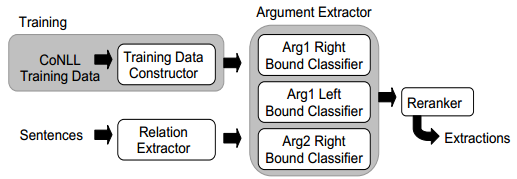
\includegraphics[scale=0.5]{../images/arglearner_architecture.png}
\caption{ArgLearner architecture training and extraction architecture}
\label{fig_arglearner_architecture}
\end{figure}

Furthermore, \textbf{Ollie} (Open Language Learning for Information Extraction)\cite{schmitz2012open} utilizes ReVerb\cite{fader2011identifying} to learn open pattern templates to guide triples extraction from sentence. Additionally, Ollie does a context analysis to extend the tuples with contextual information in order to improve precision\cite{schmitz2012open}. Its training and extraction architecture is describe in Figure \ref{fig_ollie_architecture}.

\begin{figure}
\centering
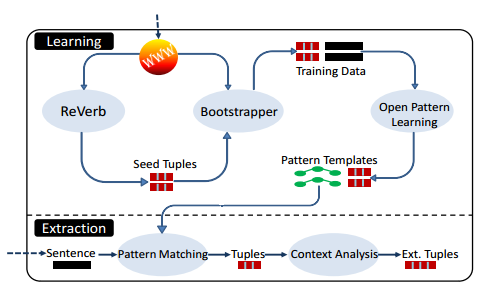
\includegraphics[scale=0.5]{../images/ollie_architecture.png}
\caption{Ollie labeling and extraction architecture}
\label{fig_ollie_architecture}
\end{figure}

One of the most research proposes new open IE system that replaces the usage of large open patterns in Ollie\cite{schmitz2012open} with a set of fewer patterns for canonically structured sentences and a classifier that learns to extract self-contained clauses from a sentence\cite{angeli2015leveraging}. This system is implemented in \textbf{Stanford OpenIE} which is also integrated in the populer open source suites, Stanford Core NLP.

\section{Proposed System}

Our proposed system also follows the pattern of three-steps\cite{etzioni2011open} method used by open IE system:

\begin{enumerate}

\item \textbf{Label}: sentences are labeled to create a training dataset for the classifier. Although most of the related systems choose to do it automatically (using heuristics or distant supervision)\cite{banko2007open}\cite{etzioni2011open}\cite\cite{schmitz2012open}, we choose to follow the method in recent research\cite{angeli2015leveraging} to manually label our training data to ensure the quality.

\item \textbf{Learn}: train a classifier using the dataset to extract dataset. We use an ensemble model, Random Forest\cite{breiman2001random}, as a classifier since it achieves the best score in our experiment.

\item \textbf{Extract}: use the classifier to extract relations (predicates) and arguments (subjects \& objects) as triples. In our case, we also do token expansion to expand the token into meaningful clause.

\end{enumerate}

As shown in the flowchart Figure \ref{fig_program_flowchart}, our system is composed of four main components: \textbf{NLP pipeline}, \textbf{triple candidate generator}, \textbf{triple selector} and \textbf{token expander}. Each of them are explained further in following subsections.

\begin{figure*}
\centering
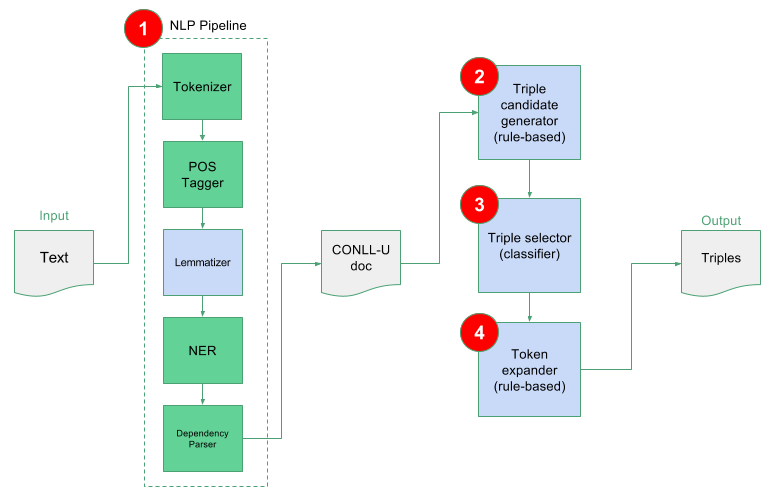
\includegraphics[width=\textwidth]{../images/program_flowchart.png}
\caption{Indonesian open domain information extraction flowchart}
\label{fig_program_flowchart}
\end{figure*}

\subsection{NLP Pipeline}

The NLP pipeline is a series of NLP tasks that annotates one or more sentences and saves them in CONLL-U\footnote{CONLL-U format description \url{http://universaldependencies.org/format.html}} format, a token-based sentence annotation format containing lemma, POS tag, dependency relation and a slot for additional annotation. The pipeline assumes that each sentence in the input document is separated by new line so preprocessing may be required. The detail of each model the pipeline are described below:

\begin{enumerate}

\item Tokenizer \\
We use default tokenizer provided by Stanford Core NLP, \verb|PTBTokenizer|\cite{manningptbtokenizer}, which mimics Penn Treebank 3 tokenizer\footnote{Penn Treebank 3 \url{https://catalog.ldc.upenn.edu/LDC99T42}}. While this tokenizer provides many options to modify its behavior, we stick to default configuration that split sentence by whitelines to get the tokens.\\

\item Part of Speech Tagger \\
We trained default Stanford Core NLP \verb|MaxentTagger|\cite{toutanova2003feature} with Indonesian universal POS tag dataset which we convert from dependency parsing dataset\footnote{UD Indonesian dataset \url{https://github.com/UniversalDependencies/UD_Indonesian}}. This POS tagger uses Max Entropy (multi-class logistic regression) classifier which yields \textbf{93.68\%} token accuracy and \textbf{63.91\%} sentence accuracy when trained using 5,036 sentences and tested with 559 sentences from the dataset. \\

\item Lemmatizer \\
The lemmatizer used in this pipeline, \verb|IndonesianLemmaAnnotator|, is implemented based on an existing Indonesian rule-based Lemmatizer\cite{suhartono2014lemmatization} with some improvements:

\begin{itemize}
\item Reimplementation in Java language
\item Usage of in-memory database to speed up dictionary lookup
\item Integration with Stanford Core NLP annotator API for reusability
\end{itemize}

This lemmatizer yields \textbf{99\%} accuracy when tested using dataset of 5,638 token-lemma pairs\footnote{Indonesian Lemmatizer \url{https://github.com/davidchristiandy/lemmatizer}}. We use lemma as one of the features for NER classifier. \\

\item Named-Entity Recognizer (NER)

Stanford NLP \verb|CRFClassifier|\cite{finkel2005incorporating}, a linear chain Conditional Random Field (CRF) sequence models, is trained using a dataset containing 3,535 Indonesian sentences with 5 entity class: Person, Organization, Location, Quantity and Time. When tested using 426 sentences, this models achieves 0.86 precision, 0.85 recall and \textbf{0.86} F1-score. The dataset itself is a combination between dataset from Faculty of Computer Science, University of Indonesia and a public dataset\footnote{Indonesian NER \url{https://github.com/yusufsyaifudin/indonesia-ner}}. \\

\item Dependency Parser

We relied on Stanford NLP \verb|nndep.DependencyParser|\cite{chen2014fast}, to annotate dependency relation of each token in the sentence. We train this transition-based neural network model using a Indonesian universal dependencies dataset of 5,036 sentences and 3,093 Indonesian word embedding\footnote{Indonesian word embedding \url{https://github.com/yohanesgultom/id-openie/blob/master/data/parser-id.embed}} (vector representation of words). Tested with 559 sentences, this model scores \textbf{70\%} UAS (Unlabeled Attachment Score) and \textbf{46\%} LAS (Labeled Attachment Score).

\end{enumerate}

The output of the pipeline is a CONLL-U document containing annotated sentence such as Figure \ref{fig_conllu_example}. The document becomes an input for next model, the triple candidate generator which is described in Section \ref{Triple Candidates Generator}. Since the annotations that are directly used by following process are POS tag, named entity and dependency relation, we estimate that the accuracy of this NLP pipeline is \textbf{65.30\%} which comes from the average of POS tagger sentence accuracy, NER F1-score (in percent) and dependency parser LAS. Additionally, this pipeline is built by extending Stanford Core NLP classes and packaged as single Java program (JAR) to improve reusability.

\begin{figure}
\centering
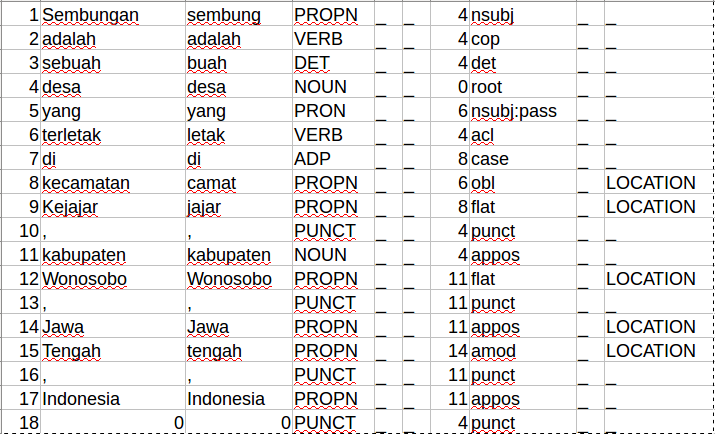
\includegraphics[scale=0.35]{../images/conllu_example.png}
\caption{Example of CONLL-U sentence annotation format}
\label{fig_conllu_example}
\end{figure}

\subsection{Triple Candidates Generator} \label{Triple Candidates Generator}

% Similar to TextRunner Self-Supervised Learner but doesn't automatically label triples

Triple candidates generator is used to extract relation triples candidates from CONLL-U document produced by NLP pipeline. It uses a set of rules listed in Table \ref{table_triple_candidate_generation_rules} to extract relations (predicates) and arguments (subjects and predicates) from the sentence. The results of triples extraction are not always the positive or valid relation triples so, unlike TextRunner\cite{banko2007open}, we cannot use them directly as training data for triple selector/classifier.

For example, applying the rules to an annotated sentence in Figure \ref{fig_conllu_example} will generate these 17 triples candidates where only five of them are valid triples (check-marked):

\begin{itemize}
\item (Sembungan, adalah, desa) \ding{51}
\item (Sembungan, adalah, terletak)
\item (Sembungan, adalah, kecamatan)
\item (Sembungan, adalah, kabupaten)
\item (Sembungan, adalah, Jawa)
\item (Sembungan, adalah, Tengah)
\item (Sembungan, adalah, Indonesia)
\item (Sembungan, terletak, kecamatan) \ding{51}
\item (Sembungan, terletak, kabupaten) \ding{51}
\item (Sembungan, terletak, Jawa) \ding{51}
\item (Sembungan, terletak, Tengah)
\item (Sembungan, terletak, Indonesia) \ding{51}
\item (desa, terletak, kecamatan)
\item (desa, terletak, kabupaten)
\item (desa, terletak, Jawa)
\item (desa, terletak, Tengah)
\item (desa, terletak, Indonesia)
\end{itemize}

In order to build a training data for the triple selector, we used triple candidates generator to generate 1,611 triple candidates from 42 sentences. As part of the label step, we manually label \textbf{132 positive} and \textbf{1,479 negative} triples which we use to train binary classifier as triple selector in the learn step.

During the extraction step, triple candidates generator is used in the system to extract unlabeled candidates from CONLL-U document. These unlabeled triples will be labeled by trained triple selector as described in  (referring to flowchart in Figure \ref{fig_program_flowchart}).

% Triple candidate generation rules
\begin{table}[!t]
\renewcommand{\arraystretch}{1.5}
\caption{Triple candidate generation rules}
\label{table_triple_candidate_generation_rules}
\centering
\begin{tabular}{l p{6cm}}
\hline
\textbf{Type} & \textbf{Condition} \\
\hline
Subject & Token's POS tag is either PROPN, NOUN, PRON or VERB \\
\space & Token is not "yang" nor "adalah" \\
\space & Token's dependency is neither "compound" nor "name" \\
\space & Token's dependency is either "compound" or "name" but separated by more than 2 tokens from its head \\
\hline
Predicate & Token's position is after Subject \\
\space & Token's POS tag is either VERB or AUX \\
\hline
Object & Token's position is after Subject and Predicate \\
\space & Token's POS tag is either PROPN, NOUN, PRON or VERB \\
\space & Token is not "yang" nor "adalah" \\
\space & Token's dependency is neither "compound" nor "name" \\
\space & Token's dependency is either "compound" or "name" but separated by more than 2 tokens from its head \\
\end{tabular}
\end{table}


\subsection{Triple Selector}  \label{Triple Selector}

Triple selector is a machine learning classifier trained using manually labeled dataset of valid and invalid relation triples. For example, given the input of 17 candidates in Section \ref{Triple Candidates Generator}, the selector will label the five check-marked triples as true and label the rest as false.

We use Random Forest\cite{breiman2001random}, an ensemble methods that aggregate classification results from multiple decision trees, as the model for the classifier. We use the Scikit-Learn\footnote{scikit-learn: machine learning in Python \url{http://scikit-learn.org}} implementation of Random Forest with following configuration:

\begin{itemize}
\item Decision tree criterion: Gini Impurity
\item Minimum number of samples to split tree node: 5 samples
\item Maximum features used in each tree: 4 (square root of the number of features)
\item Maximum trees depth: 8
\item Number of trees: 20
\item Class weight: balanced (prediction probability is multiplied by the ratio of training samples)
\end{itemize}

We discover the configuration by using Grid Search\cite{wasserman2015grid}, an exhaustive search algorithm to find optimal hyper-parameters, to find the best F1 score for Random Forest classifier using dataset described in Section \ref{Triple Candidates Generator}. 

We extract 17 features described in Table \ref{table_models_features} from each triple candidates. These features are based on POS tag, named-entity and dependency relation, instead of shallow syntactic features used by TextRunner or ReVerb\cite{banko2007open}\cite{etzioni2011open}. Every nominal features are also encoded and normalized along with the whole dataset by removing the mean and scaling to unit variance in order to improve the precision and recall of the classifier.

\begin{table}[!t]
\renewcommand{\arraystretch}{1.5}
\caption{Triple selector features}
\label{table_models_features}
\centering
\begin{tabular}{r l}
\hline
\textbf{\#} & \textbf{Triple Features} \\
\hline
1 & Subject token's POS tag \\
2 & Subject token's dependency relation \\
3 & Subject token's head POS tag \\
4 & Subject token's named entity \\
5 & Subject token's distance from predicate \\
6 & Subject token's dependency with predicate \\
7 & Predicate token's POS tag \\
8 & Predicate token's dependency relation \\
9 & Predicate token's head POS tag \\
10 & Predicate token's dependents count \\
11 & Object token's POS tag \\
12 & Object token's dependency relation \\
13 & Object token's head POS tag \\
14 & Object token's named entity \\
15 & Object token's dependents count \\
16 & Object token's distance from predicate \\
17 & Object token's dependency with predicate \\
\end{tabular}
\end{table}

During the train step, we use the dataset to train triple selector and save the best model as binary file. This model is included in the system to be use during the extraction step.

\subsection{Token Expander}

Instead of using lightweight noun phrase chunker\cite{banko2007open}, our system uses rule-based token expander to extract relation or argument clauses. While having different objective and approach, this token expander works similarly to Clause Selector in Stanford Open IE\cite{angeli2015leveraging} where the algorithm starts from a token then decides whether to expand to its dependents. Instead of using machine learning model like Clause Selector, it uses simple heuristics based on syntactical features (POS tag, dependency relation and named-entity) described in Table \ref{table_token_expansion_rules_s_o} and Table \ref{table_token_expansion_rules_p} to determine whether to: (1) expand a token to its dependent, (2) ignore the dependent or (3) remove the token itself. For example, token expander will expand check-marked triples in Section \ref{Triple Candidates Generator} into:

\begin{itemize}
\item (Sembungan, adalah, desa)
\item (Sembungan, terletak di, kecamatan Kejajar)
\item (Sembungan, terletak di, kabupaten Wonosobo)
\item (Sembungan, terletak di, Jawa Tengah)
\item (Sembungan, terletak di, Indonesia)
\end{itemize}

% Token expansion rules for Subject or Object token
\begin{table}[!t]
\renewcommand{\arraystretch}{1.5}
\caption{Token expansion rules for Subject or Object token}
\label{table_token_expansion_rules_s_o}
\centering
\begin{tabular}{r p{6cm} l}
\hline
\textbf{\#} & \textbf{Condition for Subject or Object Token} & \textbf{Action} \\
\hline
1 & If dependent's relation to the token  is either “compound”, “name”  or “amod” & Expand \\
2 & If dependent has same named entity as the token & Expand \\
3 & If dependent and the token are wrapped by quotes or double quotes  & Expand \\
4 & If the head is a sentence root & Ignore \\
5 & If dependent's POS tag is CONJ or its form is either “,” (comma) or “/” (slash) & Ignore \\
6 & If dependent's POS tag is either “VERB” or “ADP” & Ignore \\
7 & If dependent has at least one dependent with “ADP” POS tag & Ignore \\
8 & If the first or last token in expansion result has “CONJ” or “ADP” POS tag & Remove \\
9 & If the first or last index of expansion result is an incomplete parentheses symbol & Remove \\
10 & If the last index of expansion result is “yang” & Remove \\
11 & Else & Ignore \\
\hline
\end{tabular}
\end{table}

\begin{table}[!t]
\renewcommand{\arraystretch}{1.5}
\caption{Token expansion rules for Predicate token}
\label{table_token_expansion_rules_p}
\centering
\begin{tabular}{r p{6cm} l}
\hline
\textbf{\#} & \textbf{Condition for Predicate Token} & \textbf{Action} \\
\hline
1 & If dependent is “tidak” & Expand \\
2 & Else & Ignore \\
\hline
\end{tabular}
\end{table}

During the label step, token expander is used to make manual annotation process easier. We label a triple candidate as valid only if it makes sense after being expanded to clause. For example, \textit{(Sembungan, terletak, kecamatan)} doesn't seem to make sense before expanded to \textit{(Sembungan, terletak di, kecamatan Kejajar)}.

\section{Experiments} \label{Experiments}

In this research, we report two experiments. The first one shows the performance comparison of four classifiers in selecting valid triples from given candidates. While the second one shows the scalability of our system (using the best classifier) extracting triples from documents (unannotated). Both experiments are run on an Ubuntu 15.04 64-bit, Intel Core i7 5500U (dual cores), DDR3 8 GB RAM, SSD 250 GB machine.

In the first experiment, we chose four classifiers each representing unique characteristics: 

\begin{enumerate}
\item Linear Logistic Regression\cite{fan2008liblinear} (linear model)
\item Polynomial Support Vector Machine (SVM)\cite{chang2011libsvm} (nonlinear model)
\item Multi-Layer Perceptron (MLP)\cite{hinton1989connectionist} with 2 hidden layers (20 and 10 ReLU\cite{nair2010rectified} neurons)
\item Random Forest\cite{wasserman2015grid} (ensemble decision trees)
\end{enumerate}
  
We use the manually annotated triple selector dataset described in Section \ref{Triple Candidates Generator} to cross-validate\cite{kohavi1995study} (k-Fold with $k=3$) the four classifiers. Since open IE systems requires both precision and recall\cite{angeli2015leveraging}, we choose F1 score to determine the best classifier for triple selector. The result of this experiment is shown by Figure \ref{fig_models_performance} and Table \ref{table_models_performance} where Random Forest achieves the highest F1 score 0.58.

\begin{figure}
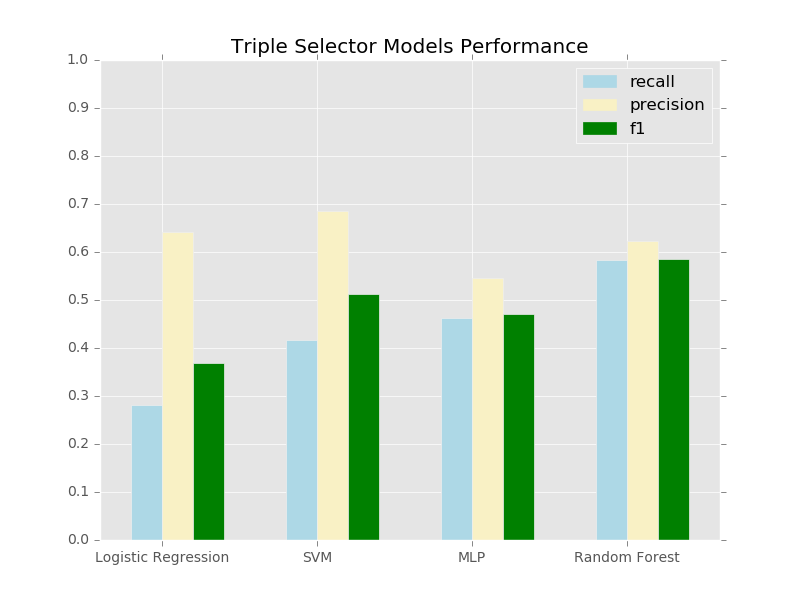
\includegraphics[scale=0.4]{../images/models_performance.png}
\caption{Triple selector models performance comparison chart}
\label{fig_models_performance}
\end{figure}

\begin{table}[!t]
\renewcommand{\arraystretch}{1.5}
\caption{Triple selector models performance}
\label{table_models_performance}
\centering
\begin{tabular}{l r r r}
\hline
\textbf{Model} & \textbf{P} & \textbf{R} & \textbf{F1} \\
\hline
Logistic Regression & 0.64 & 0.28 & 0.36 \\
SVM & \textbf{0.68} & 0.41 & 0.51 \\
MLP & 0.54 & 0.46 & 0.47 \\
Random Forest & 0.62 & \textbf{0.58} & \textbf{0.58} \\
\hline
\end{tabular}
\end{table}

In the second experiment, we evaluate the performance of our system by extracting triples from three documents with different number of sentences, measuring the total execution time and calculating the average execution time per sentence. The result in Table \ref{table_system_extraction_time} shows that the lowest execution time (or fastest execution time) is 0.014 seconds when processing document of 5,593 sentences.

\begin{table}[!t]
	\renewcommand{\arraystretch}{1.5}
	\caption{System end-to-end extraction time}
	\label{table_system_extraction_time}
	\centering
	\begin{tabular}{l p{1.2cm} p{1.2cm} p{1.2cm}}
		\hline
		\textbf{Sentences} & \textbf{Triples Extracted} & \textbf{Total Time (s)} & \textbf{Time per Sentence (s)} \\
		\hline
		2 & 7 & 6.1 & 0.800 \\
		138 & 429 & 11.3 & 0.082 \\
		5,593 & 19,403 & 78.6 & 0.014 \\
		\hline
	\end{tabular}
\end{table}

\section{Analysis}

The first experiment shows that all classifiers are still having problem learning the pattern of triples when cross-validated using $k=3$ which means two thirds of our dataset is insufficient to cover the patterns in other one third part. The dataset also suffers unbalance 1:11 ratio of positive and negative samples which is caused by lack of efficiency in triple candidates generator. To solve this issue, we plan to annotate more sentences to increase the coverage and improve the efficiency of triple candidates generator. The low performance of linear logistic regression indicates that this problem is not linearly separable. The random forest performs better than other nonlinear models (SVM and MLP) because it is easily tuned to balance the precision and recall by changing the number and the depth of decision trees.

We are also aware that the heuristics used in triple candidates generator and token expander are still limited to explicit pattern. For instance, triple candidate generator can not extract relations \textit{(kecamatan Kejajar, terletak di, Jawa Tengah)} and \textit{(Jawa Tengah, terletak di, Indonesia)} from the sentence in Figure \ref{fig_example_io_openie} yet. In the future research, we plan to improve the model to extract implicit patterns while keeping the number of negative candidates. The token expander is having problem in expanding token to implicitly expected clauses such as \textit{"seorang pelatih sepak bola"} from \textit{"seorang pelatih dan pemain sepak bola"} or \textit{"satu buah torpedo"} from \textit{"satu atau dua buah torpedo"}. We expect there will be more patterns that need to be considered in order to properly expand the token so further research on effective model to achieve this is required. Also, in order to properly evaluate the performance of these components, we need to create test datasets for both triple candidates generator and token expander.

Additionally, through the second experiment, we also find that our system average extraction performance is 0.014 seconds/sentence (for 5,593 sentences document) which is still comparable to TextRunner\cite{banko2007open}. Therefore, in contrast to the argument proposed in the related work\cite{banko2007open}\cite{etzioni2011open}, this experiment shows that the heavy linguistic tasks such as dependency parsing doesn't cause performance drawback in big document, assuming the average number of sentences in document do not exceed 5,593.

\section{Conclusion}

This paper introduces an open domain information extraction system for Indonesian text using basic NLP pipelines and combination of heuristics and machine learning models. The system is able to extract meaningful domain-independent relations from Indonesian sentences to be used as document representation or document understanding task. Additionally, the source code and datasets are published openly\footnote{Paper source code \url{https://github.com/yohanesgultom/id-openie}} to improve research reproducibility.

In the future, we plan to improve the performance of our system finding better heuristics for triple candidates generator to reduce the negative samples. We also plan adding more training data for triple selector to improve the precision and recall score. We also need to create dataset for triple candidates generator and token expander in order to properly evaluate further improvement of both components. We also consider adding confidence level in the output of every phases (NLP pipelines, candidate generator, triple selector, token expander) and including them as features and/or heuristics may also improve the overall performance of the system.

% conference papers do not normally have an appendix

% use section* for acknowledgment
%\ifCLASSOPTIONcompsoc
  % The Computer Society usually uses the plural form
%  \section*{Acknowledgments}
%\else
  % regular IEEE prefers the singular form
%  \section*{Acknowledgment}
%\fi

\bibliographystyle{IEEEtran}
\bibliography{../pustaka}

% that's all folks
\end{document}
